% Neovarch Agent technical report.
% Build: see docs/paper/README.md (pdflatex + bibtex; figures from figures/make_figures.py).
\documentclass[11pt]{article}

\usepackage[a4paper,margin=2.4cm]{geometry}
\usepackage[T1]{fontenc}
\usepackage[utf8]{inputenc}
\usepackage{lmodern}
\usepackage{microtype}
\usepackage{amsmath}
\usepackage{graphicx}
\usepackage{booktabs}
\usepackage{tabularx}
\usepackage{multirow}
\usepackage{xcolor}
\usepackage{enumitem}
\usepackage{caption}
\usepackage[numbers,sort&compress]{natbib}
\usepackage{adjustbox}
\usepackage{tikz}
\usetikzlibrary{positioning,arrows.meta,fit,backgrounds}
\usepackage[hidelinks]{hyperref}
\usepackage{url}

\definecolor{nvred}{HTML}{C8101A}
\definecolor{nvdark}{HTML}{8F0A0A}
\definecolor{nvink}{HTML}{1A1A1A}
\setlist{itemsep=1pt,topsep=3pt}
\captionsetup{font=small,labelfont=bf}
\newcommand{\code}[1]{\texttt{\hyphenchar\font=`\-\relax #1}}
\setlength{\emergencystretch}{3em}
\urlstyle{same}

\title{\textbf{Neovarch Agent: A Local-First, Phone-Controlled Coding Agent\\with a Lean, Verification-Gated Harness}\\[4pt]
\large Technical Report}
\author{Muhammad Maftuh\\
NeovarchLabs, Bandung, Indonesia\\
\small\url{https://github.com/Maftuuh1922/neovrach_Agent}}
\date{October 2026\\\small Describes \code{main} at commit \code{88a67fc} (v1.4.8 plus the unreleased Tempest lean turns, PR \#59)}

\begin{document}
\maketitle

\begin{abstract}
\noindent Neovarch Agent is an open-source AI agent that runs on the user's own Windows or Linux PC and can be driven
from an Android phone. The PC hosts a Python agent core and an Electron desktop; the phone is a remote control
only, paired once by QR code and connected over the local network, Tailscale, or an optional end-to-end encrypted
relay. The agent loop is wrapped in \emph{Tempest}, a deterministic harness layer that adds no extra model calls: it keeps the
prompt prefix byte-stable for provider caching, offloads and masks old tool output, syntax-checks edits, runs the project's tests
before a turn may end, checkpoints files, and checks unverified ``done'' claims. Two later additions target cost per task:
\emph{codemode}, in which the model writes one short Python program that calls several tools under the same safety gates,
and \emph{lean turns}, which batch work and avoid extra verification turns for failures that were already present. We describe the architecture,
its lineage (the desktop is derived from Hermes Desktop; the core is original code that speaks the same wire protocol),
and the safety model. We then report the benchmarks we actually ran, all with a single model (\code{deepseek-v4-flash-0731}
on a free provider quota). On a 10-task set run twice, Neovarch (lean, codemode) solved 20/20 tasks with 62 model calls,
327k prompt tokens, \$0.039 equivalent cost, and 473\,s, against Hermes Agent at 20/20 with 95 calls, 677k tokens, \$0.080, and 1322\,s;
Pi solved 19/20 and Codex CLI 18/20. This set is at ceiling: it separates efficiency, not capability. A harder set was cut off by the
quota after 3 tasks (Neovarch 3/3, Hermes 3/3, Pi 3/3, Codex 1/2). The samples are small and the conclusions are limited accordingly.
\end{abstract}

\begin{center}
\begin{minipage}{0.92\linewidth}
\small
\textbf{Abstrak (Bahasa Indonesia).}
Neovarch Agent adalah agen AI sumber terbuka yang berjalan di PC milik pengguna sendiri (Windows atau Linux) dan bisa
dikendalikan dari ponsel Android. PC menjalankan core agen berbasis Python dan aplikasi desktop Electron; ponsel hanya
berfungsi sebagai remote, dipasangkan sekali lewat kode QR dan tersambung lewat jaringan lokal, Tailscale, atau relay
opsional yang terenkripsi ujung ke ujung. Loop agen dibungkus \emph{Tempest}, lapisan harness deterministik yang tidak menambah panggilan model:
menjaga awalan prompt tetap sama persis agar cache penyedia terpakai, memindahkan dan menyamarkan output alat lama,
mengecek sintaks hasil edit, menjalankan tes proyek sebelum giliran boleh selesai, membuat checkpoint file, dan menindak klaim
``selesai'' yang belum terbukti. Dua tambahan berikutnya menyasar biaya per tugas: \emph{codemode}, yaitu model menulis satu
program Python pendek yang memanggil banyak alat lewat gerbang keamanan yang sama, dan \emph{lean turns}, yang menggabungkan
langkah kerja dan tidak menambah giliran verifikasi untuk kegagalan yang memang sudah ada sebelumnya. Laporan ini menjelaskan arsitektur,
asal-usulnya (desktop diturunkan dari Hermes Desktop; core ditulis sendiri namun memakai protokol yang sama), dan model keamanannya.
Kami melaporkan hanya benchmark yang benar-benar dijalankan, semuanya dengan satu model (\code{deepseek-v4-flash-0731} lewat kuota
gratis). Pada set 10 tugas yang dijalankan dua kali, Neovarch (lean, codemode) lulus 20/20 dengan 62 panggilan model,
327 ribu token prompt, biaya ekuivalen \$0,039, dan 473\,detik; Hermes Agent 20/20 dengan 95 panggilan, 677 ribu token, \$0,080,
dan 1322\,detik; Pi 19/20 dan Codex CLI 18/20. Set ini sudah mentok di plafon, sehingga hanya membedakan efisiensi, bukan kemampuan.
Set yang lebih sulit terhenti karena kuota habis setelah 3 tugas (Neovarch 3/3, Hermes 3/3, Pi 3/3, Codex 1/2).
Sampelnya kecil dan kesimpulannya terbatas.
\end{minipage}
\end{center}

\section{Introduction}

Terminal coding agents such as Codex CLI~\citep{codexcli}, Aider~\citep{aider}, Pi~\citep{pi}, and general agents such as
Hermes Agent~\citep{hermesagent} run a model in a loop with tools for the shell and the file system, in the style of
ReAct~\citep{yao2023react}. Neovarch Agent takes the same basic loop and makes three different product choices:

\begin{enumerate}
\item \textbf{The PC is the core.} The agent, its sessions, memory, skills, and settings live on the user's own machine
  (\code{\textasciitilde/.neovarch}). There is no Neovarch server; only the conversation sent to the model provider the user chose leaves the PC.
\item \textbf{The phone is a remote.} The Android app has no agent runtime and no API keys. It pairs with the PC and then chats,
  approves risky commands, and watches tasks and PC status.
\item \textbf{The harness should be cheap.} The project's working constraint is free or low-cost models, so most harness
  work aims to finish the same task with fewer model calls and fewer tokens, without extra model calls of its own.
\end{enumerate}

\noindent This report documents the system as of commit \code{88a67fc} and reports the benchmarks that were run during
its development, with their limits. It is written by the project's developer; it is not an independent evaluation.

\paragraph{Contributions.}
(i)~A description of a local-first agent with a phone remote, including its pairing and transport design (\S\ref{sec:arch});
(ii)~Tempest, a deterministic, cache-preserving harness layer with verification gates, plus codemode and lean turns (\S\ref{sec:tempest});
(iii)~a same-model comparison against Hermes Agent, Codex CLI, and Pi, with exact numbers and a frank account of what they do not show (\S\ref{sec:eval}).

\section{Lineage and licensing}
\label{sec:lineage}

Neovarch Agent began as a phone client for Hermes Agent~\citep{hermesagent} by Nous Research. The current code base has
two parts with different provenance, as recorded in the repository's \code{NOTICE} file:

\begin{itemize}
\item \textbf{Desktop (\code{desktop/})} is derived from Hermes Desktop (Electron, Vite, React/TypeScript), forked from
  \code{apps/desktop} and \code{apps/shared} of the Hermes Agent repository at commit \code{61b7f95}, MIT License, Copyright (c) 2025
  Nous Research. The original notices are kept in \code{desktop/LICENSE} and \code{desktop/NOTICE}. The desktop was later redesigned
  and rebranded.
\item \textbf{Core (\code{core/})}, the \code{neovarch} CLI, agent loop, tools, sessions, memory, skills, and the
  \code{neovarch serve} gateway, is original code written for Neovarch and contains no Hermes code. Up to the 1.2.x
  releases the desktop drove the Hermes Python core itself; an original core replaced it in v1.3.0. Its design and wire protocol are inspired by Hermes
  Agent: the gateway re-implements, from that project's public behaviour, the JSON-RPC-over-WebSocket and REST shapes the derived desktop and the phone speak
  (including the \code{HERMES\_BACKEND\_READY} readiness line and the \code{X-Hermes-Session-Token} header name), so the derived desktop works unchanged.
  The agent's working method and self-improvement skill adapt Hermes Agent's publicly documented guidance in the project's own words;
  no prompt text or code was copied.
\item Other credited sources: the Findings$\to$Evidence$\to$Unknowns$\to$Next-action report structure follows REA (MIT); the PowerPoint
  feature downloads PPT Master~\citep{pptmaster} on demand; Kantor's company flow (\S\ref{sec:kantor}) is modelled on Paperclip~\citep{paperclip};
  codemode (\S\ref{sec:codemode}) cites Reason Agent~1.1~\citep{reasonagent11}.
\end{itemize}

\noindent Neovarch uses its own home directory (\code{\textasciitilde/.neovarch}) and gateway port (9319, not Hermes' 9119), and
refuses shell commands that touch a Hermes installation, so both can run on one PC. The project is MIT-licensed.

\section{System architecture}
\label{sec:arch}

\begin{figure}[t]
\centering
\begin{adjustbox}{max width=\linewidth}
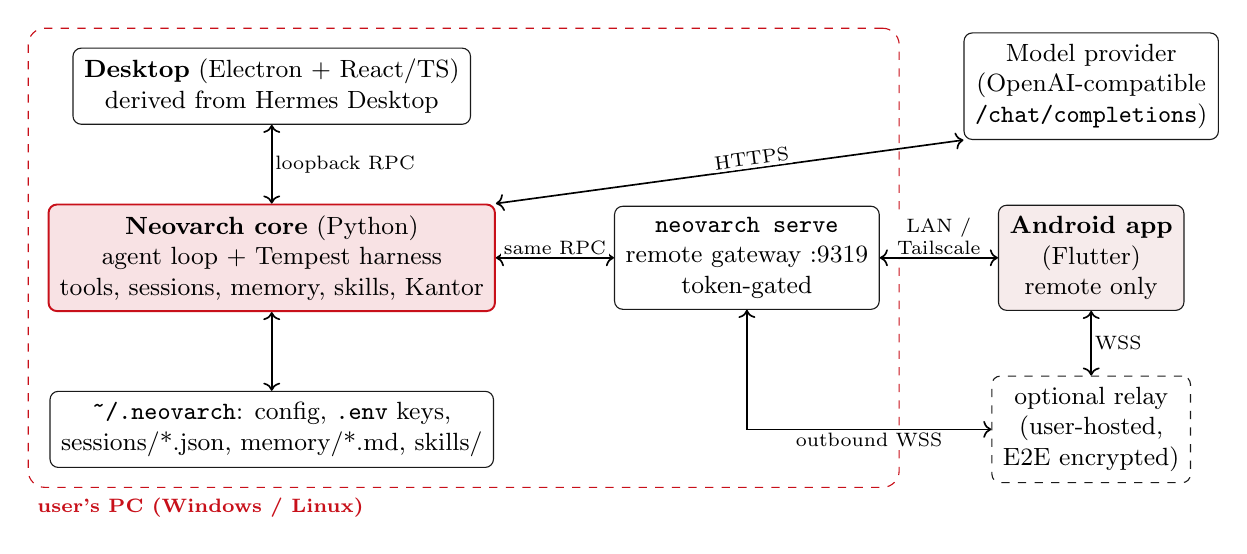
\begin{tikzpicture}[
  box/.style={draw=nvink, rounded corners=3pt, align=center, font=\small, inner sep=4pt, minimum height=0.9cm},
  core/.style={box, fill=nvred!12, draw=nvred, line width=0.7pt},
  arr/.style={-{Stealth[length=2mm]}, line width=0.6pt},
  lbl/.style={font=\scriptsize, align=center, fill=white, inner sep=1pt}]
  \node[core, minimum width=4.2cm] (core) {\textbf{Neovarch core} (Python)\\ agent loop + Tempest harness\\ tools, sessions, memory, skills, Kantor};
  \node[box, above=1.0cm of core, minimum width=4.2cm] (desk) {\textbf{Desktop} (Electron + React/TS)\\ derived from Hermes Desktop};
  \node[box, right=1.5cm of core, minimum width=2.9cm] (gw) {\code{neovarch serve}\\ remote gateway :9319\\ token-gated};
  \node[box, below=1.0cm of core, minimum width=4.2cm] (home) {\code{\textasciitilde/.neovarch}: config, \code{.env} keys,\\ sessions/*.json, memory/*.md, skills/};
  \node[box, right=1.5cm of gw, minimum width=2.3cm, fill=nvdark!8] (phone) {\textbf{Android app}\\ (Flutter)\\ remote only};
  \node[box, dashed, minimum width=2.3cm] at (phone |- home) (relay) {optional relay\\ (user-hosted,\\ E2E encrypted)};
  \node[box, minimum width=2.3cm] at (phone |- desk) (llm) {Model provider\\ (OpenAI-compatible\\ \code{/chat/completions})};
  \draw[arr, <->] (desk) -- node[lbl, right]{loopback RPC} (core);
  \draw[arr, <->] (core) -- node[lbl, above]{same RPC} (gw);
  \draw[arr, <->] (gw) -- node[lbl, above]{LAN /\\Tailscale} (phone);
  \draw[arr, <->] (relay) -- node[lbl, right]{WSS} (phone);
  \draw[arr, <->] (gw) |- node[lbl, pos=0.75, below]{outbound WSS} (relay);
  \draw[arr, <->] (core) -- (home);
  \draw[arr, <->] (core.north east) -- node[lbl, pos=0.55, above, sloped]{HTTPS} (llm.south west);
  \begin{scope}[on background layer]
    \node[draw=nvred, dashed, rounded corners=6pt, fit=(desk)(core)(home)(gw), inner sep=7pt,
      label={[font=\scriptsize\bfseries, text=nvred, anchor=north west]south west:user's PC (Windows / Linux)}] {};
  \end{scope}
\end{tikzpicture}
\end{adjustbox}
\caption{Components and trust boundary. Everything inside the dashed box runs on the user's PC. The phone holds no keys
and runs no tools; it reaches the gateway directly (LAN or Tailscale) or, if the user configures one, through a relay that only forwards encrypted frames.}
\label{fig:arch}
\end{figure}

Figure~\ref{fig:arch} shows the parts. At \code{88a67fc} the core package (\code{core/neovarch}) has about 33k lines of Python and 59 test modules.

\subsection{Core}
The core is a single Python package exposed as the \code{neovarch} command (terminal chat, one-shot \code{-q}, session
management, configuration, \code{update}) and as a gateway (\code{neovarch serve}) that the desktop and the phone talk to.
It works with any model behind an OpenAI-compatible \code{/chat/completions} endpoint (OpenAI, OpenRouter, Groq, DeepSeek, Ollama, local servers, or
router gateways). API keys sit in \code{\textasciitilde/.neovarch/.env}. The agent loop streams events (\code{message.delta}, \code{tool.start},
\code{tool.complete}, \code{message.complete} with usage and a verification status) to every attached client.
Some DeepSeek~V4 gateways occasionally return tool calls as DSML markup inside the text; the core converts that markup back into real tool calls (\code{llm.py}).

\subsection{Desktop}
The Electron desktop starts the core on loopback, renders chats, tool timelines and approvals, and hosts the settings, the Kantor
(agent office) view, the Obsidian-format Vault with a link graph, and the Pamerkan share card. For remote access it starts a second,
token-gated gateway process on port 9319 and shows the pairing QR.

\subsection{Phone remote and pairing}
The Flutter app is remote-only: no local agent, no provider settings, no local tools. Pairing works as follows:
\begin{itemize}
\item The desktop's QR carries a \emph{one-time pair token} (HMAC-signed, valid 10 minutes). It opens only the device-registration
  endpoint, which returns this phone's own session token; the core stores only its SHA-256. A successful pairing advances a pairing epoch,
  so the same QR cannot pair a second phone.
\item Devices carry \code{created\_at}/\code{last\_seen}; a device idle for \code{remote.pairing\_idle\_days} (default 30) is unpaired, and each
  device can be revoked from the desktop. Rotating the gateway secret cuts every phone at once.
\item Transport is JSON-RPC 2.0 over WebSocket plus a few REST routes, with a 15\,s heartbeat and exponential reconnect; on reconnect the
  phone re-attaches with \code{session.resume}, which also returns approvals still waiting.
\end{itemize}

\paragraph{Reaching the PC.} Since v1.4.7 the phone tries the PC's Tailscale~\citep{tailscale} address first (100.x IP, then MagicDNS) and then the LAN;
with the phone's VPN off it tries the LAN first. On Linux PCs with a default-deny firewall the app detects ufw or firewalld and, with the user's
authorisation (pkexec), adds a rule for private LAN ranges; the Windows side was fixed separately. A relay remains for users who set their own relay URL (Cloudflare Worker or Node/Docker, in \code{relay/}); the built-in default relay was removed in v1.4.7
because it had never been deployed. On relay links each connection derives per-direction ChaCha20-Poly1305~\citep{rfc8439} keys via HKDF-SHA256~\citep{rfc5869}
from X25519~\citep{rfc7748} static and ephemeral exchanges, with implicit counter nonces, so the relay sees only room membership, sizes and timing.
A Bluetooth transport has settings and a handshake but is not shipped.

\subsection{Tools}
Under Tempest the model sees a small, fixed set of core tool schemas: \code{shell}, \code{read\_file}, \code{write\_file}, \code{edit\_file},
\code{grep}, \code{glob}, \code{skill}, \code{memory}, \code{web\_search}, \code{web\_fetch}, \code{send\_file}, \code{plan\_update},
\code{session\_search}, \code{update\_plan}, and \code{codemode}. Rarely used tools (Kantor management, reports, PPT, Obsidian, diagrams, image questions,
\code{apply\_patch}, \code{repo\_map}, \code{task}, and others) sit behind one \code{extra\_tool} whose \code{describe} action returns a schema as a tool
result and whose \code{run} action is unwrapped into the real tool before any gate runs. Notable tools:
\begin{itemize}
\item \code{edit\_file} tolerates whitespace, indentation and smart-quote drift, accepts several edits per call, and reports the closest match on failure.
\item \code{apply\_patch} applies Codex-style V4A multi-file patches all-or-nothing; under Tempest every touched file is syntax-checked and a broken file rolls the whole patch back.
\item \code{repo\_map} builds a dependency-free (regex) symbol map ranked by how often other files reference a file, within a token budget.
\item \code{task} runs up to four read-only sub-agents in parallel, each with a fresh context and at most eight steps; only their short reports return.
\item \code{shell} keeps output on timeout and can run background jobs; \code{web\_search} needs no API key (fallback chain plus a 10-minute cache).
\end{itemize}
User-level hooks (\code{\textasciitilde/.neovarch/hooks.json}) can block or annotate tool calls; hook files inside a repository are never run.
\code{/rencana} (alias \code{/plan}) runs a read-only planning turn. Project instruction files (\code{AGENTS.md}, \code{NEOVARCH.md}, \code{CLAUDE.md}) are loaded from the git root down to the working folder.

\subsection{Sessions, memory, and skills}
Sessions are JSON files (\code{sessions/<id>.json}) on the PC that any attached client (terminal, desktop, phone) can list and resume.
\code{session\_search} queries a local SQLite FTS5 index of all saved chats, updated incrementally just before each search.
Memory is Markdown notes (\code{memory/*.md}); before an append, exact and near-duplicate lines (similarity $\geq 0.9$ against any note) are dropped,
and a reminder to save durable facts rides on the next user message every six turns or after a finished task. Skills are folders with a \code{SKILL.md};
a verified task with at least five tool calls becomes a skill offer, and per-skill use/pass/fail counts are tied to verification results.
The Vault is a real Obsidian-format vault (Markdown, wikilinks, \code{.obsidian}) linked to projects and sessions.

\subsection{Kantor: an agent office}
\label{sec:kantor}
Kantor (``office'') lets the main agent run a small company of agent employees, each with its own persona, skills, tools, and model, which the main
agent can create, assign, and fire on the user's instruction. Following Paperclip~\citep{paperclip}, a heartbeat drives employees once a company exists (pausable from desktop and phone);
the CEO gets a strategy ticket per active goal and proposes a plan that the user, as the board, approves, sends back, or rejects; hires always go through an approval;
costs are recorded per model call and a budget hard stop interrupts the running heartbeat and files one budget approval. A live activity feed and ticket threads (comments, audit trail, heartbeat runs) are visible on both clients.
Kantor has been tested with mocks only, not with live model runs.

\subsection{Updates and Pamerkan}
\code{neovarch update} and a desktop button update in place: a git install is fast-forwarded only (it refuses dirty trees, detached heads, and diverged branches),
dependencies are reinstalled, and a failed or interrupted update resets to the previous commit (\code{--rollback} undoes the last one). Other installs re-run the
official installer for the latest release, or open the release page for AppImage/\code{.deb}. Pamerkan is a shareable usage card whose radar (coding, research, slides,
browser, automation, tokens) is computed only from local session and usage files on log scales against fixed references; with no data it shows an empty card rather than invented numbers.

\section{Safety and approvals}
\label{sec:safety}
\begin{itemize}
\item \textbf{Approval modes.} \code{approvals.mode} is \code{ask} (default) or \code{off}. In \code{ask}, a shell command matching a list of dangerous patterns
  (recursive/forced delete, \code{sudo}, disk formatting, \code{dd} to devices, shutdown, broad \code{chmod}/\code{chown}, force-push or \code{reset --hard},
  piping a download into a shell, \code{kill -9}, fork bombs, \code{DROP TABLE}) waits for the user, who can answer once, for the session, always, or deny,
  on the desktop, in the phone's approval tab, or from an Android notification (300\,s timeout).
\item \textbf{Workspace boundary.} A command whose working directory is outside the chat's workspace always asks, even with approvals off.
\item \textbf{Codemode sandboxing.} Codemode programs run in a separate isolated Python process with a minimal environment, a timeout (default 60\,s, max 300\,s),
  and on Linux/macOS CPU, memory (1\,GB) and file-size limits (no direct file writes). Network is off unless both the call and the config allow it. This is a guard, not a full
  security boundary: the real boundary is that every side effect goes through \code{tools}, and therefore through the gates above.
\item \textbf{Gateway exposure.} The desktop's own backend binds to loopback; remote access is a separate token-gated process. Over plain-\code{http} LAN the token
  is visible to anyone sniffing that network, which the protocol documentation states openly; \code{https}/\code{wss} and the encrypted relay avoid this.
\item \textbf{Hooks and extras.} Only user-owned hook files run. Optional extras such as Obsidian are installed from official sources and only with consent.
\end{itemize}

\section{The Tempest harness}
\label{sec:tempest}

Tempest has been the default ``brain'' since v1.4.7 (\code{agent.harness\_mode: legacy} restores the older loop). Its rule is that every mechanism is
deterministic and adds \emph{zero} model calls; feedback from the harness rides as a tail on the next user message and never edits the system prompt.

\subsection{Phase 1: cache-stable context and verification}
\begin{enumerate}[label=\arabic*.]
\item \textbf{Stable prefix.} Date/time and per-message notes leave the system prompt; config changes after the session starts are appended as a note. Tool schemas
  are canonical (sorted names and keys), and up to four \code{cache\_control} breakpoints are placed for Anthropic-compatible endpoints. A lint checks that the prefix never changes between calls.
\item \textbf{Offload and masking.} Large tool results go to a file, leaving head, tail and path in context; read-only results are clipped around the query instead.
  At 50\% of the context window, old tool outputs are swapped for placeholders that keep the path to the full text, and only beyond a second threshold is a deterministic
  structured summary used. This follows the finding that simple observation masking is competitive with LLM summarization~\citep{lindenbauer2025complexity}.
\item \textbf{Edit gates.} Writes to \code{.py}, \code{.json}, \code{.js} and \code{.ts} are syntax-checked and a broken file is restored. Available static checkers (builtin, ruff, pyright, mypy, tsc)
  run before and after a change, and only \emph{new} diagnostics block.
\item \textbf{Verification gate.} When a turn that changed files wants to end, the detected test command runs; on failure the model is asked to fix it, at most a fixed number of retries, then the turn stops with an escalation note.
  This is a harness-run analogue of self-reflection loops such as Reflexion~\citep{shinn2023reflexion}.
\item \textbf{Shadow checkpoints.} A separate git directory snapshots files before the first modifying tool and at the end of a turn, tagged green or red by the gate; when the gate gives up, files return to the last green checkpoint (\code{/rewind} by hand). The user's own git is untouched.
\end{enumerate}

\subsection{Phase 2: learning loop and claim gate}
Session search, memory reminders with deduplication, and skills learned from verified multi-step tasks are described above. The \emph{claim gate} gives one hidden
correction to a final answer that says ``done'', ``fixed'' or ``tests pass'' without a successful execution after the last code edit; if the claim is still unbacked, the answer is marked
as unverified. Each turn reports \code{verification} $\in$ \{verified, unverified, failed, none\}.

\subsection{Prompt diet}
The first prompt was cut from about 11.4k to 5.5k tokens by sending only skill \emph{names} (matching descriptions ride on the user message) and only the core tool schemas, with the
rest behind \code{extra\_tool}. The tools array stays byte-identical within a session.

\subsection{Codemode}
\label{sec:codemode}
In codemode the model writes one short Python program that calls tools through a \code{tools} object (\code{tools.read\_file(...)}, \code{tools.parallel([...])},
\code{tools.describe(...)}) and prints only what it needs. One model call can then search, read several files, and run tests. The idea follows CodeAct~\citep{wang2024codeact}
and Cloudflare's Code Mode~\citep{varda2025codemode}, and the repository credits Reason Agent~1.1~\citep{reasonagent11} as its direct inspiration. What is specific to Neovarch is that every inner call takes the
same path as a direct call: approvals, workspace boundary, plan mode, syntax checks and checkpoints, hooks, disabled tools, memory dedup, and the evidence ledger the claim gate reads.
Within one \code{parallel}, read-only tools run concurrently and modifying tools run in order. Limits: 64 tool calls per program, 16 per \code{parallel}, 12,000 characters of output.
The codemode schema is static and part of the core tool list, so caching is unaffected; it costs about 650 extra tokens per request.

\subsection{Lean turns}
Logs from a live benchmark on 2026-10-14 showed where extra turns came from: the verification gate ran \code{pytest -x}, so in a repository that was already red, fixing one old failure exposed the next
old failure as if it were new and forced repair rounds; the gate also asked for a skill patch mid-task; skill hints ordered a skill read before starting; and the working method encouraged separate planning
turns and re-reads. Lean turns (\code{agent.tempest\_lean}, default on) change this:
\begin{itemize}
\item a working method that asks for large batched steps, no re-reads, one verification, and the exact answer format requested; skill hints become offers;
\item a full-suite gate without \code{-x} that separates pre-existing failures from new ones by test id; old failures the answer already mentions cost no retry;
\item tests run automatically after an edit, and the result is attached to the edit's tool result, so the model can answer directly and the end-of-turn gate can reuse it;
\item a small project snapshot on the first message; a read cache (an unchanged file still on the wire returns a one-line pointer, a changed one returns a diff when shorter);
\item recovery of DSML tool calls emitted as text.
\end{itemize}

\section{Evaluation}
\label{sec:eval}

We report only benchmarks that were run, with numbers copied from their result files. All live comparisons use one model, \code{deepseek-v4-flash-0731}, through the free quota of the
Intern-AI Discovery API, with each agent pointed at a local relay that forwards requests and records the provider's \code{usage} for every call. The arms were:
Neovarch (Tempest lean; codemode, the shipped default, and a variant with parallel reads but no codemode), Hermes Agent at commit \code{0e427d78} (toolsets terminal, file, todo; memory and background review off; at most 40 iterations),
Codex CLI 0.80.0 (\code{exec}, chat-completions wire API, approvals and sandbox bypassed), and Pi 0.73.1 (print mode, no session, extensions, or skills). Every arm got the same prompt, repository, and grader.

\paragraph{Metrics.} \emph{Pass} is decided by a deterministic grader (tests, hidden tests, or format-tolerant answer checks). \emph{Calls} and \emph{prompt tokens} come from the provider's usage fields.
\emph{Equivalent cost} is $(\text{prompt}+\text{completion tokens}) \times \$0.115$ per million: a flat reference price for comparison, because the quota was free; it is not a bill and ignores cache discounts.
\emph{Wall time} is summed per arm; arms shared one provider and ran in parallel lanes, so time is indicative only.

\subsection{Ten-task set}

The tasks run against a small shop package with tests: four questions about the code (\code{qna-discount-callers}, \code{qna-todos}, \code{qna-config-usage}, \code{qna-failing-tests}), an API summary
(\code{api-summary}), and five code changes (\code{fix-tax-rounding}, \code{rename-line-total}, \code{fix-inventory-offbyone}, \code{add-feature-low-stock-test}, \code{fix-both-and-verify}).
The repository starts with known failing tests, so agents must tell old failures from new ones. The set was run twice (rounds g1 and g2).

\paragraph{Grader fixes.} In a first pass, two tasks failed for every agent. Inspection showed the graders were at fault: \code{qna-config-usage} demanded an exact string
(\code{"CURRENCY -> tidak dipakai"}) the prompt never asked for, and \code{add-feature-low-stock-test} demanded a file named \code{tests/test\_low.py}, a name the prompt never gave.
Both graders were rewritten to check substance (every constant and its users named and \code{CURRENCY} reported unused, in any wording; a passing test of \code{.low()} with its default
limit anywhere under \code{tests/}, with no failures beyond the repository's two pre-existing ones). The same grader file is used for all arms, and both rounds were run after the fix, except
for one g1 row (Codex, \code{qna-config-usage}) that was re-graded with the final grader from its stored answer (it passes).

\begin{table}[t]
\centering
\small
\caption{Ten-task set, deepseek-v4-flash-0731, two rounds. Prompt tokens include cached tokens. Equivalent cost at a flat \$0.115/M tokens.}
\label{tab:bench10}
\begin{tabular}{llrrrrr}
\toprule
Round & Arm & Pass & Calls & Prompt tok & Equiv.\ \$ & Wall s \\
\midrule
\multirow{5}{*}{g1}
 & Neovarch lean, codemode (default) & 10/10 & 30 & 157,972 & 0.0191 & 292 \\
 & Neovarch lean, parallel           & 10/10 & 32 & 158,153 & 0.0191 & 177 \\
 & Hermes Agent                      & 10/10 & 51 & 367,723 & 0.0436 & 764 \\
 & Codex CLI                         &  9/10 & 64 & 574,493 & 0.0682 & 453 \\
 & Pi                                &  9/10 & 56 & 154,408 & 0.0192 & 502 \\
\midrule
\multirow{5}{*}{g2}
 & Neovarch lean, codemode (default) & 10/10 & 32 & 169,079 & 0.0203 & 180 \\
 & Neovarch lean, parallel           & 10/10 & 37 & 192,568 & 0.0232 & 263 \\
 & Hermes Agent                      & 10/10 & 44 & 309,561 & 0.0368 & 558 \\
 & Codex CLI                         &  9/10 & 52 & 450,639 & 0.0534 & 452 \\
 & Pi                                & 10/10 & 64 & 230,240 & 0.0286 & 491 \\
\midrule
\multirow{5}{*}{both}
 & Neovarch lean, codemode (default) & \textbf{20/20} & \textbf{62} & \textbf{327,051} & \textbf{0.0394} & 473 \\
 & Neovarch lean, parallel           & \textbf{20/20} & 69 & 350,721 & 0.0423 & \textbf{440} \\
 & Hermes Agent                      & \textbf{20/20} & 95 & 677,284 & 0.0804 & 1322 \\
 & Codex CLI                         & 18/20 & 116 & 1,025,132 & 0.1216 & 905 \\
 & Pi                                & 19/20 & 120 & 384,648 & 0.0478 & 994 \\
\bottomrule
\end{tabular}
\end{table}

\begin{figure}[t]
\centering
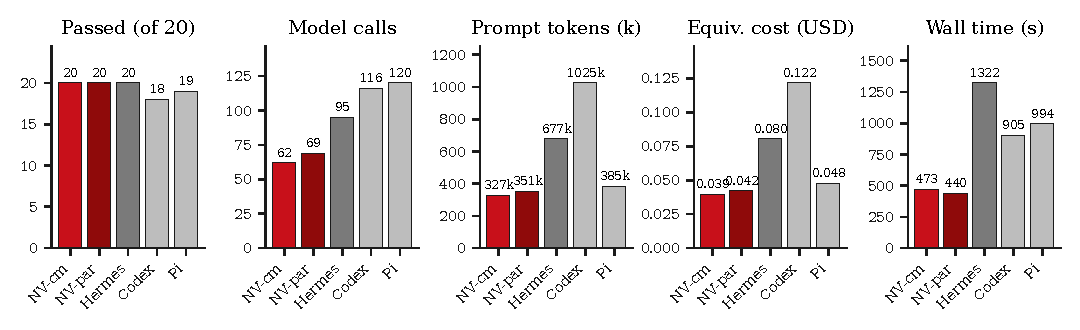
\includegraphics[width=\linewidth]{figures/bench10.pdf}
\caption{Ten-task set, both rounds combined (Table~\ref{tab:bench10}). NV-cm: Neovarch lean with codemode (default); NV-par: Neovarch lean with parallel reads.}
\label{fig:bench10}
\end{figure}

\paragraph{Results.} Table~\ref{tab:bench10} and Figure~\ref{fig:bench10} give the numbers. Neovarch's default configuration solved all 20 runs, as did Hermes Agent; Pi missed
\code{rename-line-total} once and Codex CLI missed \code{fix-tax-rounding} in both rounds. In the Codex failures the gateway forwarded DSML tool-call markup as plain text and Codex stopped;
Neovarch converts this markup back into tool calls (lean turns), so these two failures are partly a property of this provider rather than of Codex's reasoning. On efficiency, Neovarch's default used
62 calls versus Hermes' 95 ($-35\%$), 327k versus 677k prompt tokens ($-52\%$), \$0.039 versus \$0.080 equivalent ($-51\%$), and 473\,s versus 1322\,s. Pi's prompt-token total (385k) is close to
Neovarch's, with about twice as many calls. The parallel-reads variant was the fastest in wall time (440\,s) at slightly higher token use.

\paragraph{What this shows and does not show.} The pass rates are at ceiling: three arms solved everything, so this set cannot rank capability. Neovarch is ahead of Pi and Codex on pass rate here
and tied with Hermes. The efficiency gap is consistent across both rounds, but with two rounds of ten tasks we report it without significance tests.

\subsection{Harder set (partial)}

To move off the ceiling we built ten harder tasks on a separate shop repository: three bug hunts (\code{hunt-csv}, \code{hunt-atomic-place}, \code{hunt-eventbus}), a refactor
(\code{refactor-unify-revenue}), a feature (\code{feature-refund}), multiple bugs (\code{fix-multi-bugs}), performance (\code{perf-reports}), a CLI (\code{cli-export}), an API deprecation
(\code{api-rename-deprecate}), and a question (\code{qna-revenue-gap}). Code tasks are graded in a directory outside the repository with a pristine copy of the visible tests plus hidden tests, so an agent's edits to tests or
configuration cannot change the verdict. Neovarch ran from \code{88a67fc} with shipped defaults (lean, codemode); the wall limit was 900\,s per run. Round~1 got through three tasks before the free quota answered HTTP~402.

\begin{table}[t]
\centering
\small
\caption{Harder set, round 1 (partial, 3 of 10 tasks), deepseek-v4-flash-0731. Codex was not run on the third task before the quota ended. One Pi call on \code{refactor-unify-revenue} reported no usage, so Pi's token count there is a lower bound.}
\label{tab:hard}
\setlength{\tabcolsep}{4pt}
\begin{tabular}{lcccc}
\toprule
 & Neovarch & Hermes & Pi & Codex CLI \\
\midrule
\code{hunt-csv}               & pass, 7 / 57k   & pass, 7 / 65k    & pass, 20 / 168k & pass, 12 / 139k \\
\code{hunt-atomic-place}      & pass, 6 / 58k   & pass, 16 / 310k  & pass, 14 / 176k & fail (timeout), 5 / 54k \\
\code{refactor-unify-revenue} & pass, 11 / 142k & pass, 15 / 250k  & pass, 14 / 168k & not run \\
\midrule
Passed                        & 3/3 & 3/3 & 3/3 & 1/2 \\
Model calls                   & 24 & 38 & 48 & 17 \\
Prompt tokens                 & 256,959 & 624,989 & 512,675 & 193,746 \\
Equivalent \$                 & 0.034 & 0.075 & 0.063 & 0.025 \\
Wall s                        & 1158 & 1273 & 1237 & 1305 \\
\bottomrule
\end{tabular}
\\[2pt]{\footnotesize Cells: outcome, model calls / prompt tokens.}
\end{table}

\begin{figure}[t]
\centering
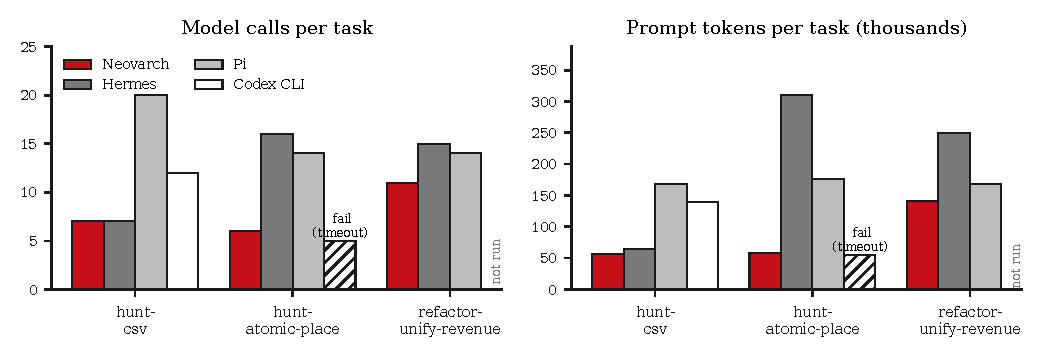
\includegraphics[width=0.95\linewidth]{figures/hard_r1.pdf}
\caption{Harder set, round 1 (partial). Hatched bar: Codex on \code{hunt-atomic-place}, which hit the 900\,s limit after 5 calls.}
\label{fig:hard}
\end{figure}

Table~\ref{tab:hard} and Figure~\ref{fig:hard} show the partial round. Three agents solved all three tasks; Codex solved \code{hunt-csv} and timed out on \code{hunt-atomic-place}. Neovarch used the fewest
calls and tokens of the agents that finished all three tasks (24 calls and 257k prompt tokens versus Hermes' 38 and 625k). Its time on \code{hunt-atomic-place} (628\,s) was the longest of the passing runs on that task, so the low call count did not translate into speed there.
Codex's totals cover only two tasks and are not comparable. Three tasks are not enough to rank pass rates; the harder set needs to be completed (\S\ref{sec:future}).

\subsection{Harness-only measurements}

Two measurements isolate the harness from model quality. They are documented in the repository and included here for completeness.
\begin{itemize}
\item \textbf{Codemode replay} (\code{core/bench/codemode\_bench.py}, 2026-10-14): the real agent loop, tools, files, pytest and Tempest run on ten local tasks while the model's choices are
  \emph{scripted} (the same hand-written trajectory per arm). Codemode needed 23 model calls versus 57 with one tool per call ($-60\%$) and 38 with parallel reads ($-39\%$); prompt tokens fell
  from 271,819 and 183,668 to 108,389, but \emph{uncached} prompt tokens fell only from 54,603 and 53,236 to 49,509 ($-9\%$ / $-7\%$), and output tokens rose by 11--13\% (Figure~\ref{fig:replay}).
  The gain is in round trips and total tokens sent (relevant for providers without caching and for per-request quotas), not in uncached input.
\item \textbf{Prompt diet} (2026-10-12): first-prompt size 11.4k $\to$ 5.5k tokens with no loss of passes in a 200-run live comparison on a different model, documented in \code{docs/tempest-vs-hermes.md}.
\end{itemize}

\begin{figure}[t]
\centering
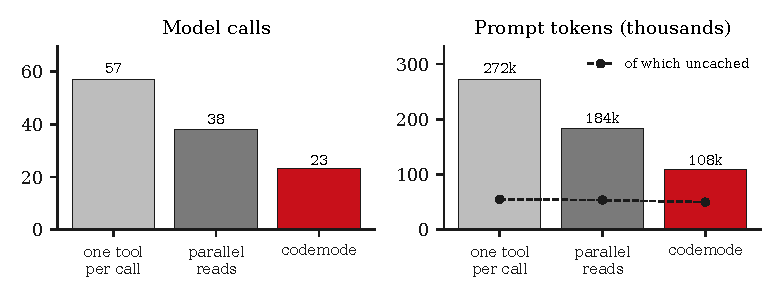
\includegraphics[width=0.72\linewidth]{figures/codemode_replay.pdf}
\caption{Codemode replay benchmark with a scripted model (harness cost only; 10 tasks, one run per arm). Dashed line: uncached prompt tokens.}
\label{fig:replay}
\end{figure}

\subsection{Provider provenance}
An earlier live run on 2026-10-14 used a commercial router (CleanAPIs, which shares a backend with RadoxAI) under the same \code{deepseek-v4-flash-0731} label. A probe of that backend showed every model label streaming
a backend model field of \code{muse-spark-1.2-contributor} together with a hidden system prompt of about 240 tokens, so that provider very likely did not serve the model it named. We infer this from the
stream and could not confirm it with the provider. Those runs are not used in this report (they were also incomplete because the credit ran out). We did not independently verify which model the Intern-AI endpoint served either;
all agents in each comparison went through the same endpoint, so the comparison is same-model even if the label is wrong, but absolute numbers should not be read as properties of DeepSeek~V4 Flash.

\section{Related work}
\label{sec:related}

\paragraph{Coding agents and harnesses.} SWE-agent~\citep{yang2024sweagent} showed that the agent--computer interface (commands, file viewer, edit format, feedback) strongly affects success on SWE-bench~\citep{jimenez2024swebench}.
OpenHands~\citep{wang2025openhands} provides an open platform for software agents with sandboxed runtimes. Aider~\citep{aider} pioneered repository maps and edit formats for terminal pair programming; Neovarch's \code{repo\_map}
is a simpler, dependency-free variant. Codex CLI~\citep{codexcli} defines the V4A patch format that \code{apply\_patch} accepts. Pi~\citep{pi,zechner2025pi} argues for a minimal harness with four tools; it is the most token-frugal baseline here.
Hermes Agent~\citep{hermesagent} is the closest relative: a general agent with skills, curated memory, background review, session search and messaging gateways. Neovarch differs mainly in doing its learning loop without extra LLM calls and in running a test gate by default.

\paragraph{Reasoning, reflection, and code actions.} ReAct~\citep{yao2023react} interleaves reasoning and tool actions; Reflexion~\citep{shinn2023reflexion} adds verbal self-reflection after failure. Tempest's gates are a deterministic,
harness-driven form of this feedback. CodeAct~\citep{wang2024codeact} showed that executable Python actions can outperform JSON tool calls; Cloudflare's Code Mode~\citep{varda2025codemode} applies the idea to MCP tools in a sandbox. Neovarch's codemode is a local variant whose distinguishing property is that inner calls keep every approval and verification gate.

\paragraph{Context management.} Lindenbauer et al.~\citep{lindenbauer2025complexity} found observation masking to match LLM summarization at about half the cost for SWE-agent; Tempest uses masking and a deterministic summary rather than an LLM summary.

\paragraph{Agent organisations.} Paperclip~\citep{paperclip} models a company of agents with org charts, goals, heartbeats, budgets and board approvals; Kantor adopts these concepts inside a single local app.

\section{Limitations}
\label{sec:limits}
\begin{itemize}
\item \textbf{One model, one provider.} All live numbers use \code{deepseek-v4-flash-0731} on one free endpoint whose served model we did not verify. Results may not transfer to other models.
\item \textbf{Small samples.} Two rounds of ten tasks and a partial round of three. One run changes a pass rate by 5--33 points. We report no confidence intervals.
\item \textbf{Ceiling.} The ten-task set is solved by three arms, so it measures efficiency only.
\item \textbf{In-house tasks and tuning.} The tasks and graders were written by the Neovarch developer, and lean turns were designed from logs of an earlier run on similar tasks. Tuning to the benchmark is therefore a real risk, which the unseen hidden tests of the harder set only partly address.
\item \textbf{Grader fixes.} Two graders were corrected after a first pass. The fixes apply to all arms and were motivated by prompts that never asked for the checked format, but post-hoc grader changes are a source of bias.
\item \textbf{Baselines.} Each baseline ran in one configuration (e.g.\ Hermes without memory or background review, Codex 0.80.0 on the chat-completions API). Other configurations may do better. Codex's two failures on \code{fix-tax-rounding} involve the provider's DSML output.
\item \textbf{Cost and time.} Equivalent cost is a flat reference price; wall time was measured on a shared endpoint.
\item \textbf{Product testing.} Many features (Kantor, update, Pamerkan, Android chat and microphone changes) were tested with unit tests, mocks, and offscreen renders, not on real Windows machines or phones; macOS and Linux ARM64 are unsupported.
\item \textbf{No public benchmark.} We have not run SWE-bench, Terminal-Bench, or similar suites (no Docker in the development sandbox).
\end{itemize}

\section{Future work}
\label{sec:future}
\begin{itemize}
\item Finish the harder set over several rounds and seeds, and add multi-session tasks that exercise session search and memory with real models.
\item Repeat the comparison on more models and providers, with a check of which model the endpoint actually serves.
\item Run public suites (SWE-bench Verified, Terminal-Bench) once a container runtime is available.
\item Show verification status and skill statistics in the desktop and phone UI; add a lifecycle for learned skills.
\item Test Kantor with live models, and test update, remote, and Android features on real hardware.
\end{itemize}

\section{Conclusion}
Neovarch Agent puts a coding agent on the user's PC, keeps the phone as a remote, and wraps the loop in a harness that adds no model calls of its own. On the benchmarks we could run, all
with one model on a free quota, its default configuration matched the best pass rate and used roughly half the tokens and equivalent cost of Hermes Agent. The evidence is narrow: one model,
small samples, a set at ceiling, and a harder set that is only started. Completing that set and adding models are the next steps.

\paragraph{Reproducibility.} The repository contains the agent at \code{88a67fc}, the codemode replay benchmark (\code{core/bench/}), and, under \code{docs/paper/data/}, the per-arm and per-run
numbers used in Tables~\ref{tab:bench10} and~\ref{tab:hard}. \code{docs/paper/figures/make\_figures.py} regenerates every chart from those files. The live-run harness (relay and CLI runners) is kept outside the repository because it installs and runs third-party agents.

\paragraph{Acknowledgements.} We thank Nous Research for publishing Hermes Agent and Hermes Desktop openly, and the authors of Codex CLI, Pi, Aider, Paperclip, PPT Master and REA, whose public work shaped parts of this project.

\bibliographystyle{plainnat}
\bibliography{references}

\end{document}
